\section{Qué se comprueba}

Después de ubicar y rutear el diseño, es necesario comprobar que la lógica pueda
funcionar con el reloj de la Basys 3. El análisis temporal estudia los caminos
que conectan los registros. Para cada uno determina si el dato producido por un
registro llega a tiempo al siguiente y permanece estable durante el intervalo
necesario.

La comprobación de setup considera el tiempo anterior al flanco de captura. El
dato debe llegar y estabilizarse antes de ese flanco. La comprobación de hold
analiza el intervalo posterior y verifica que el dato no cambie demasiado
pronto. El análisis de ancho de pulso comprueba que los niveles alto y bajo del
reloj duren el tiempo requerido por el dispositivo.

Cada camino termina en un punto de captura que el reporte denomina
\emph{endpoint}. El margen indica cuánto tiempo queda entre la llegada del dato
y el límite correspondiente a ese punto.

Vivado informa el resultado de setup mediante WNS y TNS. El WNS corresponde al
menor margen encontrado entre todos los caminos. El TNS suma únicamente los
márgenes negativos.

Para hold, el WHS representa el menor margen y el THS reúne los márgenes
negativos. En el análisis del ancho de pulso, el WPWS indica el peor margen y el
TPWS suma las violaciones.

Un valor positivo de WNS o WHS indica que incluso el peor camino analizado
cumple con la restricción. Cuando TNS o THS valen cero, no existen endpoints con
margen negativo. Esto no significa que los caminos tengan un retardo nulo.
Significa que ninguno supera el límite establecido.

El reloj se define en el archivo \texttt{basys3.xdc}. La restricción crea
\texttt{sys\_clk} con un período de \SI{10}{\nano\second}, que corresponde a
una frecuencia de \SI{100}{\mega\hertz}. A partir de esta definición, Vivado
analiza los caminos internos que comienzan y terminan en registros controlados
por ese reloj.

No todas las señales externas pueden analizarse con la misma relación temporal.
Las entradas {\color{technicalviolet}\path{btn_reset}} y
{\color{technicalviolet}\path{serial_rx}} pueden cambiar sin
estar sincronizadas con {\color{technicalviolet}\path{sys_clk}}. Por eso, el archivo
\texttt{basys3.xdc} declara una excepción desde ambos puertos hasta la primera
etapa de sus sincronizadores mediante \texttt{set\_false\_path}.

Las doce salidas tampoco poseen una relación temporal con un reloj externo. Una
corresponde a \texttt{serial\_tx} y las otras once controlan los LED. Como no
existe un reloj de captura externo asociado con \texttt{sys\_clk}, sus caminos
hasta los pines también se declaran con \texttt{set\_false\_path}.

Además de calcular los márgenes, el reporte revisa que la definición temporal
no deje partes internas del diseño sin analizar. El resultado no presenta
registros sin reloj, relojes constantes, lazos combinacionales ni endpoints
internos sin restricción.

El análisis temporal se limita a estas propiedades. No determina si el
protocolo UART interpreta correctamente una solicitud ni si el enlace USB
funciona sobre la placa. El comportamiento del protocolo se comprobó mediante
la simulación funcional. La conexión física se evalúa en la validación sobre la
Basys 3.

\section{Resultado posterior al ruteo}

Una vez definidas las restricciones, el análisis se ejecutó sobre el diseño
completamente ruteado. El archivo
\texttt{reports/timing\_summary.rpt} contiene los resultados obtenidos para el
dispositivo y la velocidad seleccionados.

\subsection{Márgenes temporales}

El reporte incluye 458 endpoints para las comprobaciones de setup y hold.
También analiza 159 endpoints para el ancho de pulso. La
figura~\ref{fig:timing-summary-vivado} muestra el resumen generado por Vivado.
Todos los márgenes son no negativos y las sumas de las violaciones permanecen
en cero.

\begin{figure}[H]
	\centering
	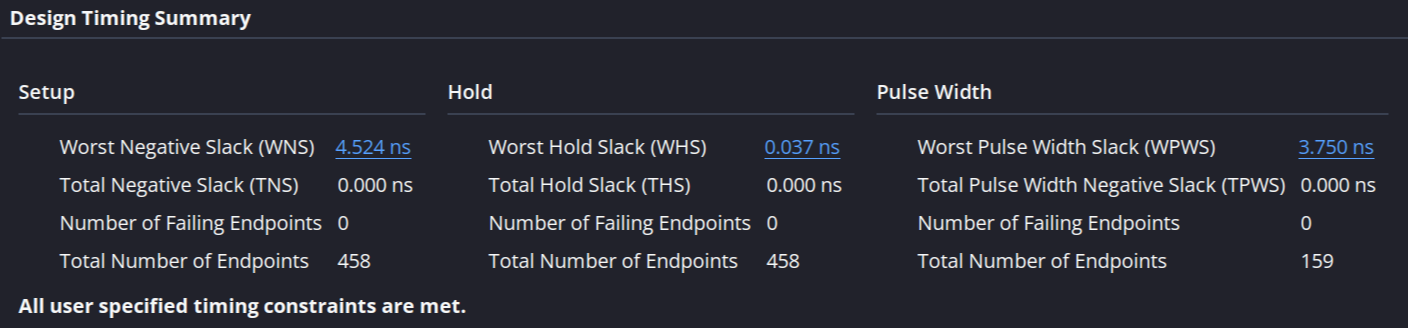
\includegraphics[width=\textwidth]{img/vivado_timing_summary.png}
	\caption{Resumen temporal del diseño posterior al ruteo.}%
	\label{fig:timing-summary-vivado}
\end{figure}

La tabla~\ref{tab:timing} reúne los valores correspondientes a los tres tipos
de análisis.

\begin{table}[H]
	\centering
	\begin{tabularx}{0.92\textwidth}{ZZZZ}
		\toprule
		\textbf{Análisis} & \textbf{Peor margen} & \textbf{Suma negativa} &
		\textbf{Endpoints} \\
		\midrule
		Setup & WNS = \SI{4.524}{\nano\second} & TNS = \SI{0}{\nano\second} & 458 \\
		Hold & WHS = \SI{0.037}{\nano\second} & THS = \SI{0}{\nano\second} & 458 \\
		Ancho de pulso & WPWS = \SI{3.750}{\nano\second} &
		TPWS = \SI{0}{\nano\second} & 159 \\
		\bottomrule
	\end{tabularx}
	\caption{Márgenes reportados después del ruteo.}%
	\label{tab:timing}
\end{table}

El peor camino de setup conserva un margen de
\SI{4.524}{\nano\second} dentro del período de
\SI{10}{\nano\second}. Esto significa que el dato llega con más de cuatro
nanosegundos disponibles antes del límite de captura.

El margen de hold es menor y alcanza \SI{0.037}{\nano\second}. Aun así,
permanece por encima de cero dentro del modelo temporal del dispositivo. Por
esta razón, el THS es igual a cero y no se informan endpoints con una violación
de hold. El análisis del ancho de pulso también cumple, con un WPWS de
\SI{3.750}{\nano\second} y un TPWS igual a cero.

Estos resultados permiten afirmar que el diseño implementado satisface las
restricciones declaradas para un reloj de \SI{100}{\mega\hertz}.

\subsection{Cruces asíncronos}

El análisis de los caminos síncronos no alcanza para evaluar las señales que
ingresan sin relación con el reloj interno. Por ese motivo también se realizó
un análisis CDC, denominado \emph{Clock Domain Crossing}. Su resultado se
guarda en \texttt{reports/cdc.rpt}. Este análisis comprueba que los cruces
entre dominios de reloj atraviesen las estructuras de sincronización previstas.

El reporte identifica exactamente dos cruces. El primero corresponde a la
liberación del reset y aparece clasificado como CDC-9. El segundo corresponde a
la entrada \texttt{serial\_rx} y aparece como CDC-3. Ambos sincronizadores
tienen una profundidad de dos etapas y poseen la propiedad
\texttt{ASYNC\_REG}. Además, los caminos desde los puertos externos están
cubiertos por las excepciones declaradas en \texttt{basys3.xdc}. El reporte
identifica ambas excepciones como \texttt{False Path}.

La figura~\ref{fig:cdc-vivado} muestra ambos cruces y permite comprobar su
clasificación, su profundidad y la excepción aplicada.

\begin{figure}[H]
	\centering
	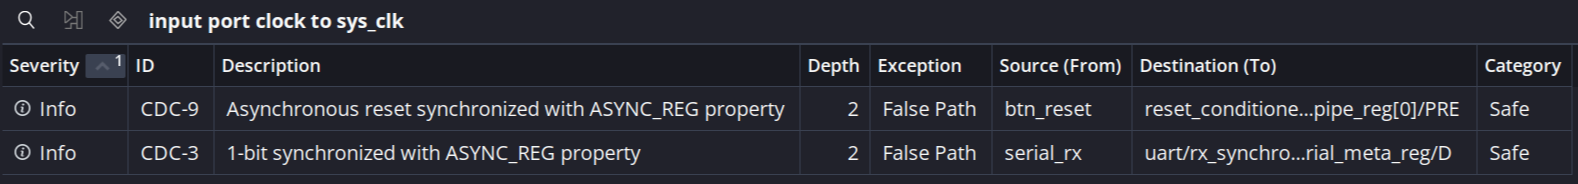
\includegraphics[width=\textwidth]{img/vivado_cdc.png}
	\caption{Cruces de dominio identificados por el análisis CDC.}%
	\label{fig:cdc-vivado}
\end{figure}

\subsection{DRC y metodología}

Después de revisar la temporización y los cruces asíncronos, se ejecutó el DRC,
o \emph{Design Rule Check}. Esta comprobación revisa las reglas del dispositivo
sobre el diseño completamente ruteado. El archivo
\texttt{reports/drc.rpt} informa \texttt{Checks found: 0}. Por lo tanto, no se
encontró ninguna violación.

La figura~\ref{fig:drc-vivado} presenta el resumen de esta comprobación.

\begin{figure}[H]
	\centering
	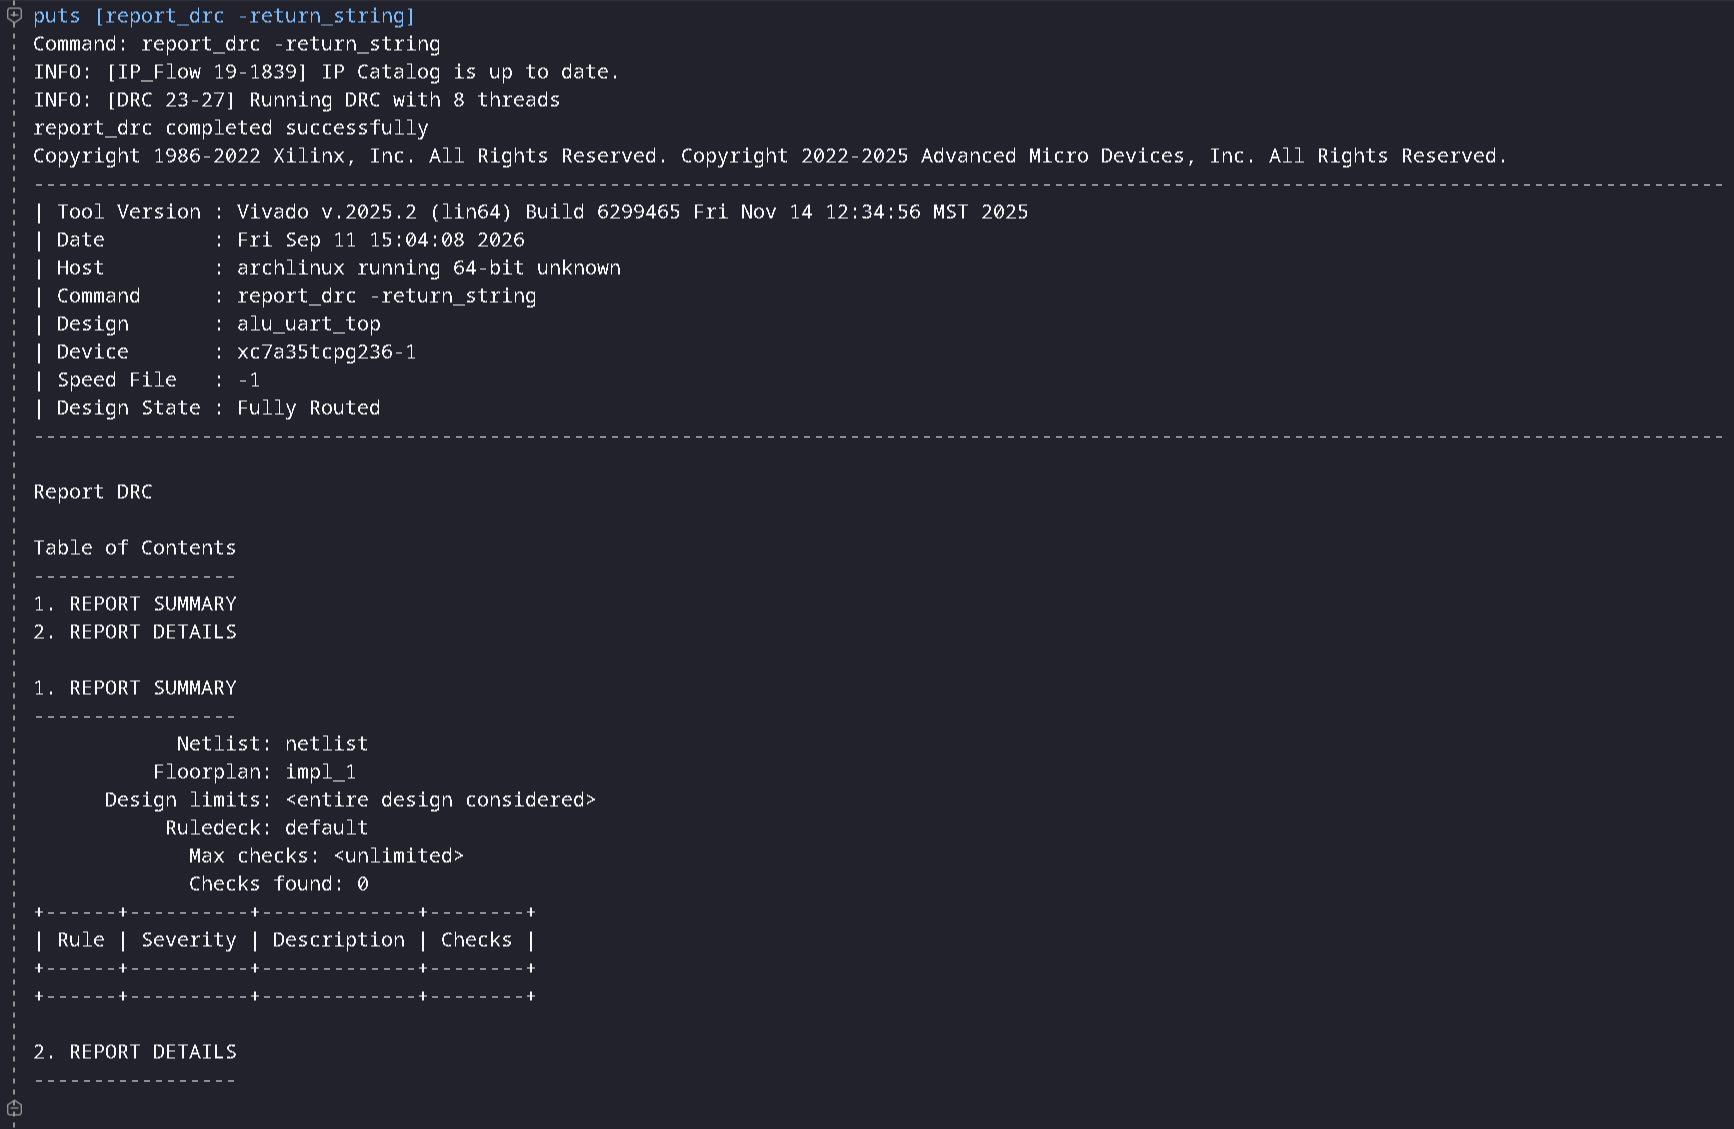
\includegraphics[width=0.72\textwidth]{img/vivado_drc.png}
	\caption{DRC del diseño completamente ruteado, sin violaciones.}%
	\label{fig:drc-vivado}
\end{figure}

Los reportes de metodología revisan otro aspecto del proceso. En este caso,
Vivado busca construcciones o decisiones que no respeten sus re\-co\-men\-da\-cio\-nes
para la síntesis y la im\-ple\-men\-ta\-ción. El archivo
\texttt{reports/synthesis\allowbreak\_methodology.rpt} no contiene hallazgos después de la
síntesis. El archivo
\texttt{reports/implementation\allowbreak\_methodology.rpt} tampoco presenta hallazgos
después de completar la implementación.

Las figuras~\ref{fig:methodology-synthesis-vivado} y
\ref{fig:methodology-implementation-vivado} muestran los resúmenes de ambos
reportes.

Las capturas permiten observar los resultados principales, pero los reportes
conservan el detalle completo de cada análisis. Los archivos utilizados son
{\color{technicalviolet}\path{reports/timing_summary.rpt}},
{\color{technicalviolet}\path{reports/cdc.rpt}},
{\color{technicalviolet}\path{reports/drc.rpt}},
{\color{technicalviolet}\path{reports/synthesis_methodology.rpt}} y
{\color{technicalviolet}\path{reports/implementation_methodology.rpt}}.

\clearpage

\begin{figure}[H]
	\centering
	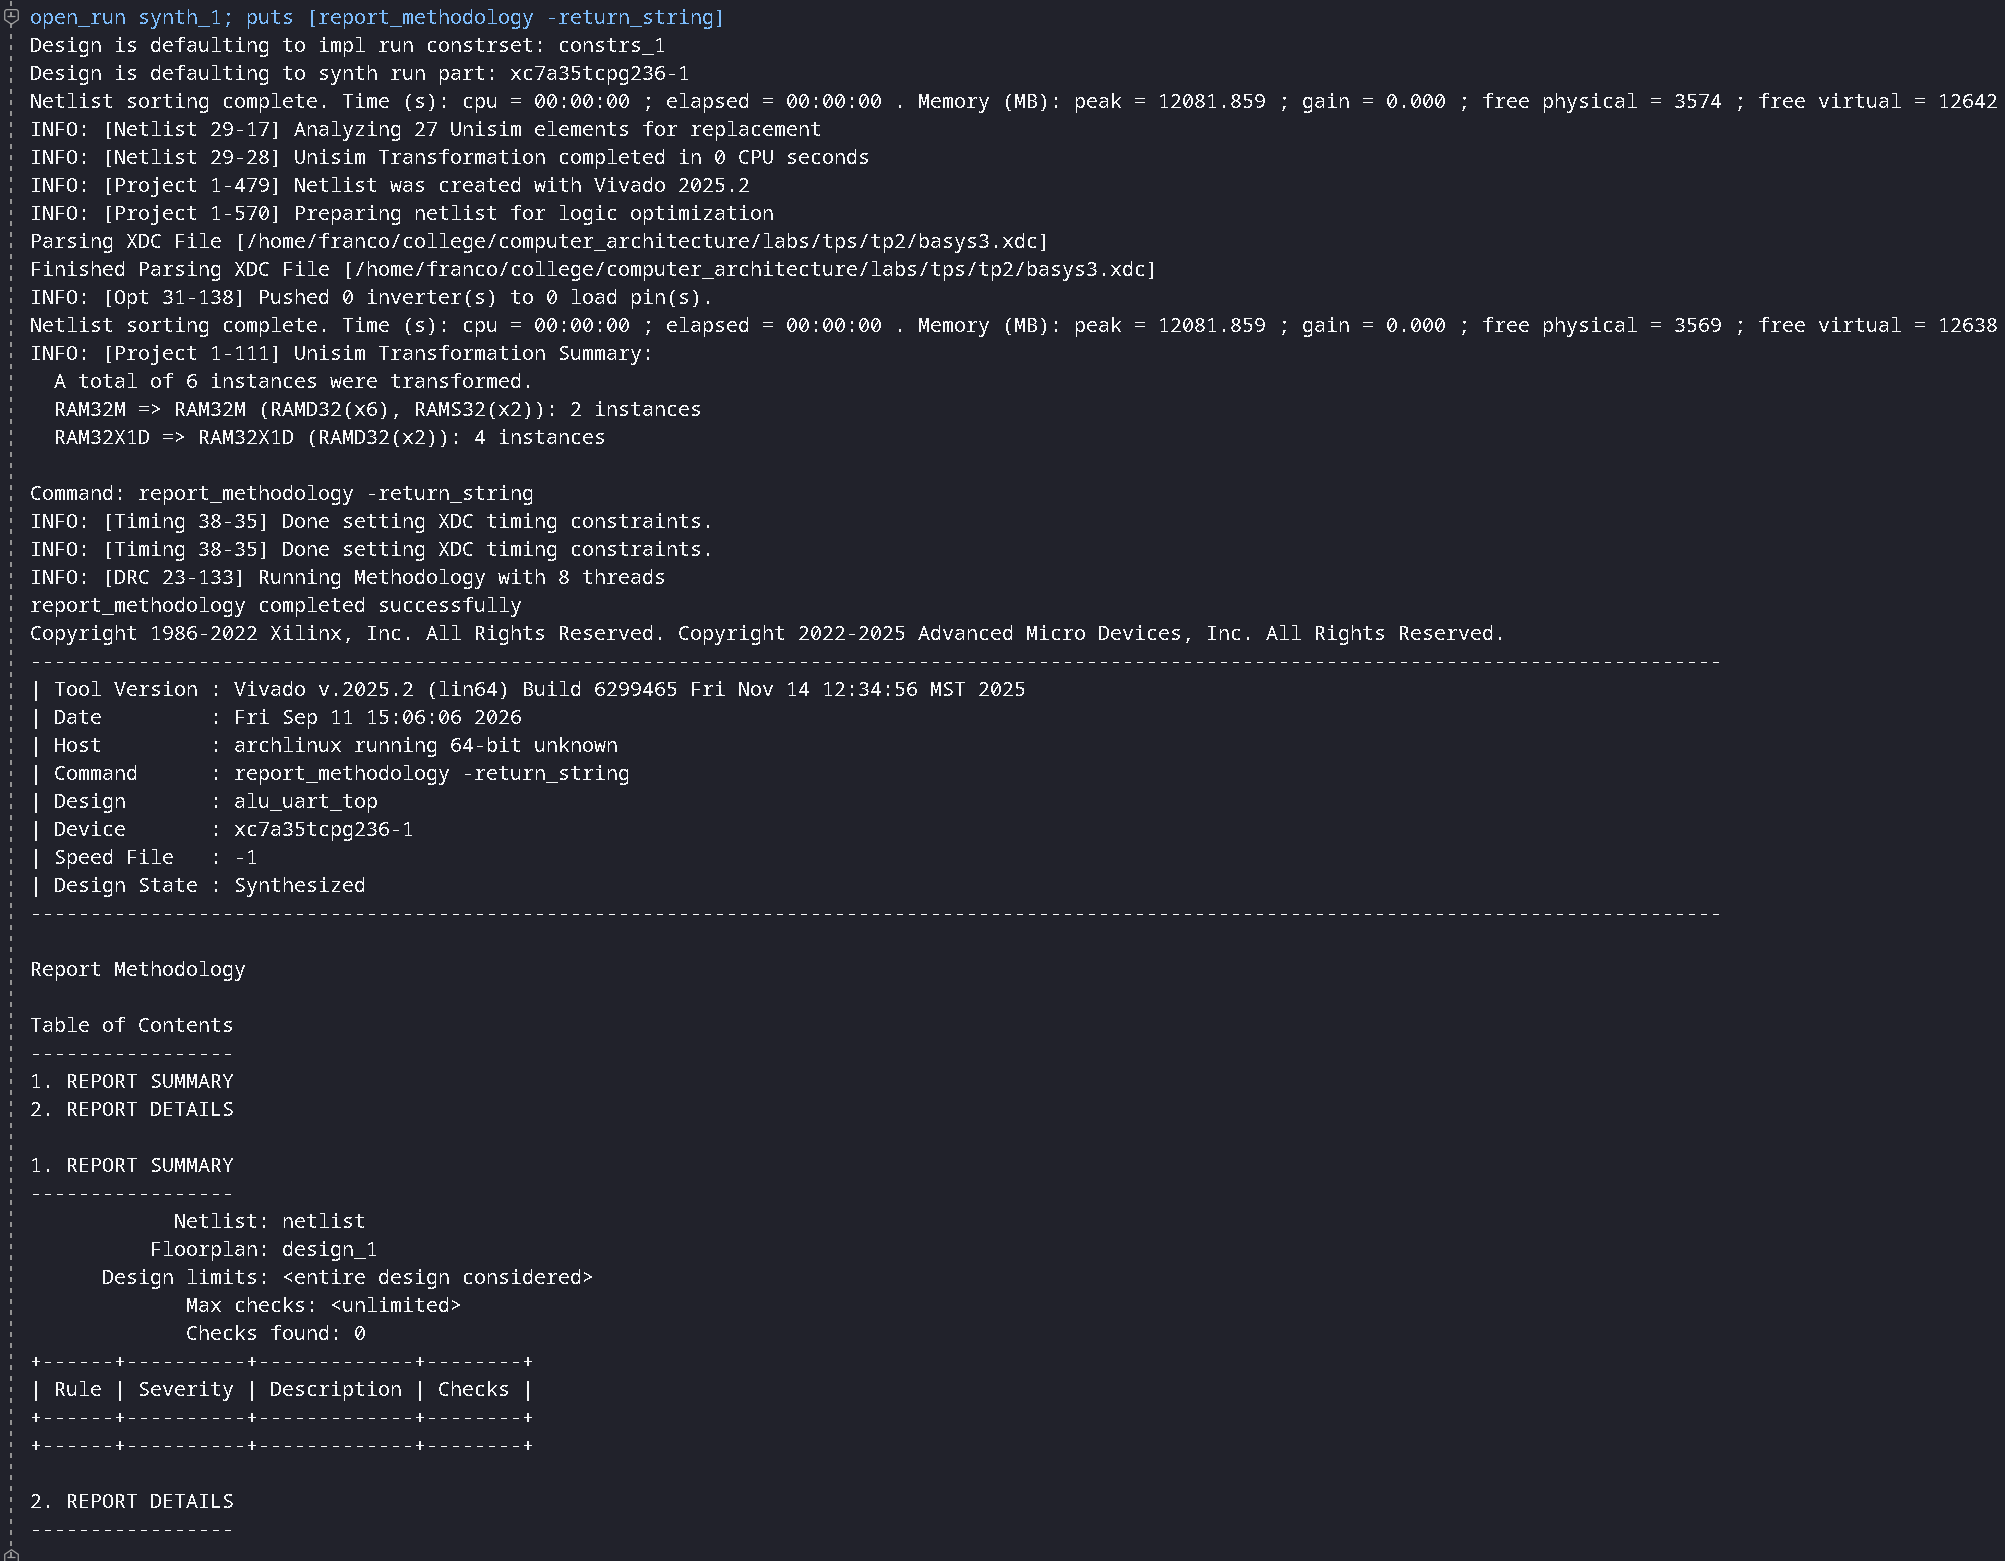
\includegraphics[width=0.74\textwidth]
	{img/vivado_methodology_synthesis.png}
	\caption{Reporte de metodología posterior a síntesis, sin hallazgos.}%
	\label{fig:methodology-synthesis-vivado}
\end{figure}

\begin{figure}[H]
	\centering
	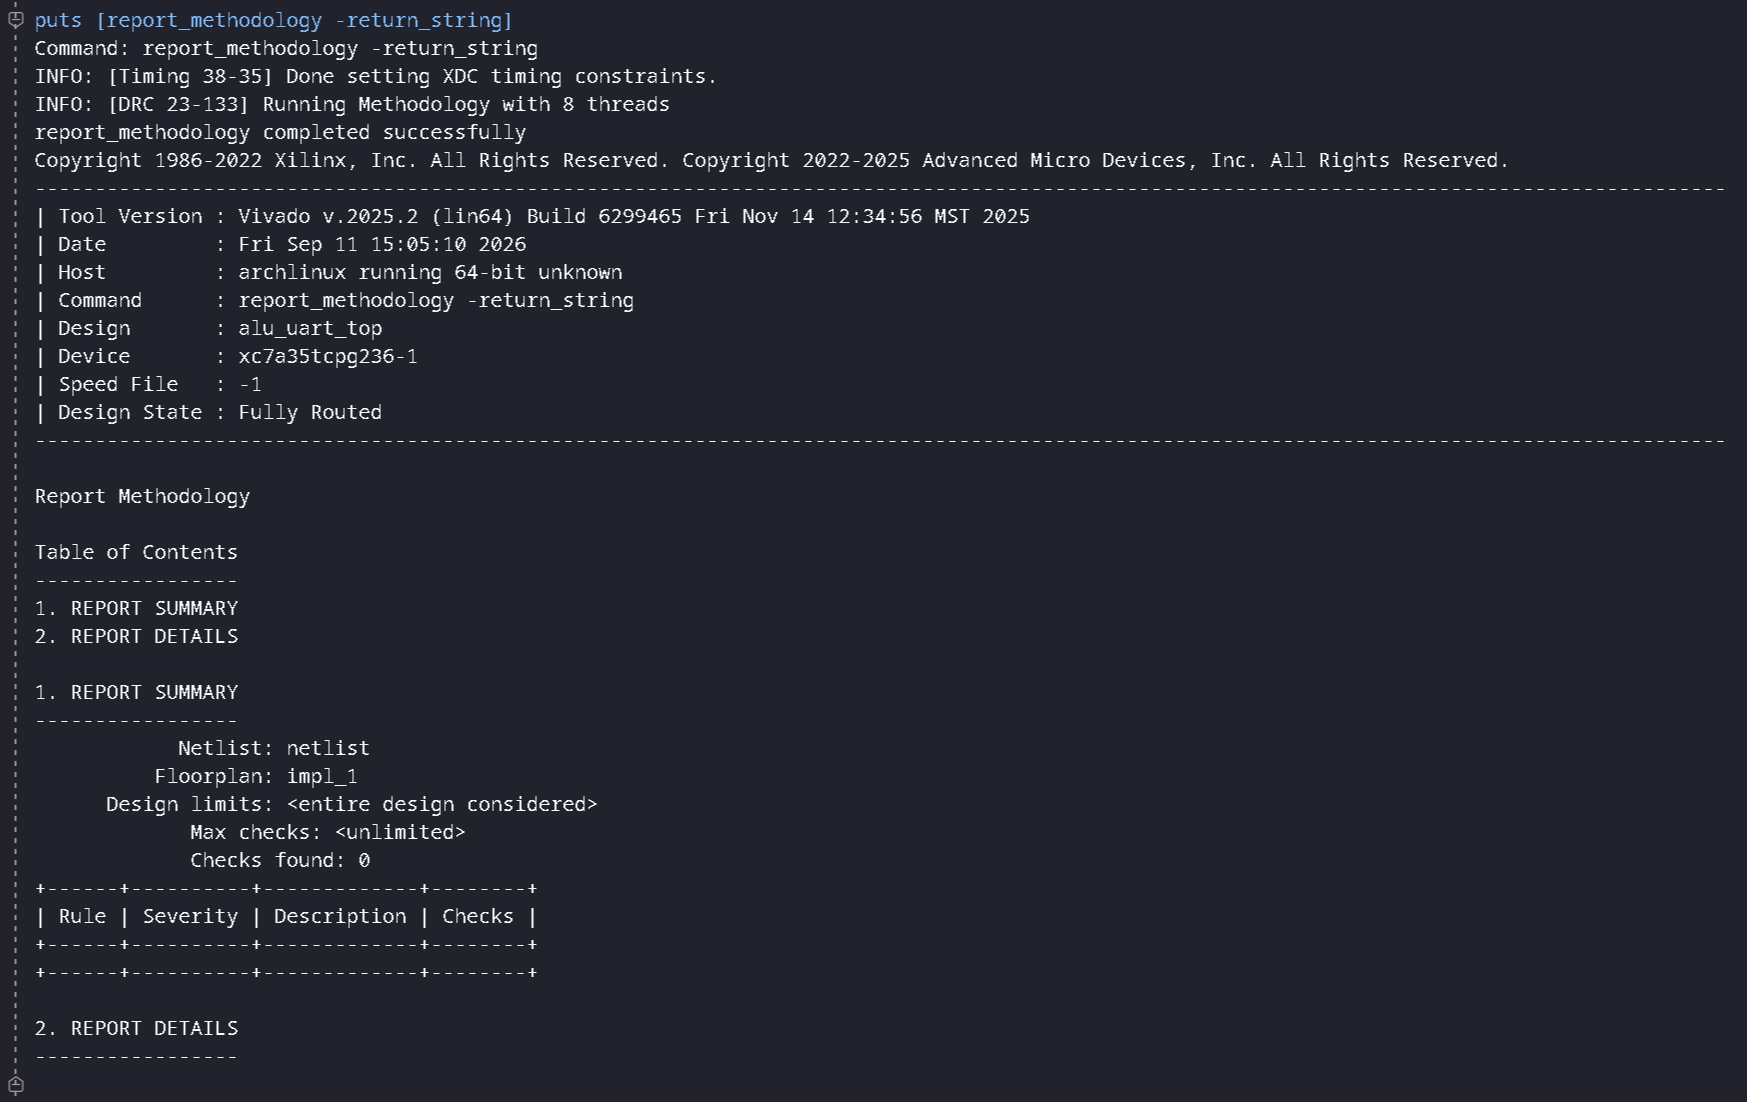
\includegraphics[width=0.82\textwidth]
	{img/vivado_methodology_implementation.png}
	\caption{Reporte de metodología posterior a implementación, sin hallazgos.}%
	\label{fig:methodology-implementation-vivado}
\end{figure}
